\documentclass{article}
\title{Unmixing detrital age distributions: a direct solution}
\author{Pieter Vermeesch\\University College London\\\texttt{p.vermeesch@ucl.ac.uk}}
\usepackage{graphicx,caption,fullpage,natbib}
\usepackage[hidelinks]{hyperref}
\begin{document}
\maketitle

\begin{abstract}
Detrital geochronology can be used to quantify sediment budgets by
estimating the proportions in which a set of known sources contribute
to a sedimentary sink, such as a river downstream of a
confluence. Existing `top-down' unmixing algorithms solve this inverse
problem by iterative search, either exhaustively testing all mixing
proportions in 1\% increments or sampling them at random. Their
computational cost grows exponentially with the number of
sources. They also rely on heuristic dissimilarity measures that lack
a firm theoretical basis and can give inconsistent results depending
on which measure is chosen. This paper presents a direct solution to
the top-down unmixing problem. Because mixing of frequency
distributions is a linear operation, the problem can be expressed in
matrix form using empirical cumulative distribution functions and
solved by least squares, subject to the constraint that the
proportions sum to one. The solution is unique and is mathematically
equivalent to minimising the Cram\'{e}r--von Mises distance between
the observed and predicted distributions, so no kernel smoothing or
choice of objective function is needed. Its speed makes bootstrap
resampling practical, which yields confidence intervals that capture
sampling uncertainty in both sources and sink. Tests on simulated
binary mixtures of normal distributions show that the method remains
accurate even when the sources overlap strongly. Applied to a
published detrital zircon U–Pb dataset from central California, the
method gives confidence intervals that encompass the full range of
results from the exhaustive search under five different dissimilarity
functions. The Cramér–von Mises statistic also serves as a diagnostic
for identifying sinks that the specified sources cannot adequately
explain. As with any top-down approach, the results are only as
reliable as the assumption that all relevant sources have been
identified, and they describe the dated mineral phase rather than
total sediment contributions. The algorithm is implemented in the
\texttt{R} package \texttt{IsoplotR}.
\end{abstract}

\section{Introduction}\label{sec:intro}

Consider the confluence of two rivers draining catchments with
contrasting geological histories, and hence distinct detrital zircon
U--Pb age distributions. Downstream of the confluence, the detrital
zircon U--Pb age spectra form a mixture of the two input signals, with
mixing proportions determined by the relative contributions of each
branch to the zircon budget of the main river. If the zircon
concentrations of both branches are known, these mixing proportions
can be used to constrain the sediment budget of the river
network. Solving this inverse problem is of considerable interest to
sedimentary geologists, as it provides an opportunity to quantify
sediment budgets using detrital geochronology. \citet{sharman2017}
distinguish between top-down unmixing, in which the sources are known,
and bottom-up unmixing, in which they are unknown. This paper focuses
exclusively on the top-down problem because the bottom-up problem has
no unique solution \citep{saylor2019}.\medskip

Existing algorithms solve the top-down problem using iterative search
strategies to find the mixing proportions that minimise the misfit
between the observed and predicted age distributions. These algorithms
are suboptimal in two respects. First, they are computationally
inefficient. \citet{sharman2017} exhaustively search all possible
mixing proportions in 1\% increments, whereas \citet{sundell2017} use
a Monte Carlo approach without a convergence criterion. Both
approaches exhibit exponential time complexity: the computational cost
of estimating the mixing proportions of a $k$-component mixture scales
with the $(k-1)$\textsuperscript{th} power of the number of possible
proportions. Second, existing unmixing algorithms quantify the misfit
between observed and predicted distributions using heuristic measures,
such as `likeness' and the `cross-correlation of probability density
plots'. These measures lack a firm theoretical foundation and have
been shown to be problematic in limiting cases such as the application
to high precision data \citep{vermeesch2018b}.\medskip

This paper presents a direct solution to the unmixing problem that
addresses both limitations. Section~\ref{sec:solution} shows that
mixing frequency distributions is a linear problem that can be
expressed in matrix form and solved using least squares
estimation. This approach is mathematically equivalent to minimising
the Cram\'{e}r--von Mises distance between the observed and predicted
distributions. Section~\ref{sec:examples} applies the new algorithm to
simulated and published datasets to demonstrate its effectiveness. The
examples also illustrate how the results can be used to identify
problematic datasets for which the underlying model assumptions are
violated. The new algorithm has been added to \texttt{IsoplotR}
\citep{vermeesch2018c} for immediate use in detrital studies
(Section~\ref{sec:IsoplotR}).

\section{A direct solution to the unmixing problem}\label{sec:solution}

The unmixing problem can be cast as a linear system of three matrices,
using the following definitions:

\begin{description}
\item{$k$:} the number of sediment sources (e.g. $k=2$ in
  Figure~\ref{fig:algorithm});
\item{$W_j$;} the contribution of the $j$\textsuperscript{th} source
  to the sink, where $W_k = 1 - \sum_{j=1}^{k-1} W_j$
  (Figure~\ref{fig:algorithm}d);
\item{$n$:} the sample size of the sink;
\item{$t_i$:} the $i$\textsuperscript{th} sample (date) of the sink
  (with $1\leq{i}\leq{n}$);
\item{$X_{i,j}$:} the cumulative probability of $t_i$ under the
  empirical cumulative distribution function of source $j$
  (Figure~\ref{fig:algorithm}e).
\item{$Y_{i} = (2i-1)/2n$}, which is essentially the empirical
  cumulative probability of $t_i$ in the sink
  (Figure~\ref{fig:algorithm}f).
\end{description}

Using these definitions, the mixing problem can be written as a linear
matrix expression:

\begin{equation}
  \left[
  \begin{array}{@{}c@{~}c@{~}c@{~}c@{~}c@{}}
    X_{1,1} & \ldots & X_{1,j} & \ldots & X_{1,k} \\
    \vdots & \ddots & \vdots & \ddots & \vdots \\
    X_{i,1} & \ldots & X_{i,j} & \ldots & X_{i,k} \\
    \vdots & \ddots & \vdots & \ddots & \vdots \\
    X_{n,1} & \ldots & X_{n,j} & \ldots & X_{n,k} \\
  \end{array}
  \right]
  \left[
    \begin{array}{@{}c@{}}
      W_{1} \\
      \vdots \\
      W_{j} \\
      \vdots \\
      W_{k}
    \end{array}
    \right]
  =
  \left[
  \begin{array}{@{}c@{}}
    Y_{1} \\
    \vdots \\
    Y_{i} \\
    \vdots \\
    Y_{n}
  \end{array}
  \right]
  \mbox{~or~}
  X\,W = Y
    \label{eq:unmix}
\end{equation}

It is worth noting that this matrix formulation is similar to the
non-negative matrix factorisation approach introduced by
\citet{saylor2019} to solve the bottom-up unmixing problem. There are
two key differences between their approach and the direct solution
presented here.  A first difference is that \citet{saylor2019}'s $X$
and $Y$ are populated with density estimates, whereas the direct
solution uses cumulative probabilities. This avoids the need for
kernel smoothing. The second difference is that both $X$ and $W$ are
unknown in \citet{saylor2019}'s bottom-up formulation, whereas $X$ is
known and only $W$ needs to be estimated in the top-down
problem. Consequently, Equation~\ref{eq:unmix} has a unique solution,
obtained by minimising the sum of squared residuals between $Y$ and
$XW$, subject to the constraint that $\sum_{j=1}^k W_j=1$. Several
methods can be used to solve Equation~\ref{eq:unmix}, including
Lagrange multipliers and non-negative least squares algorithms
\citep{lawson1995}. Unlike non-negative matrix factorisation, this
least squares problem has a unique solution.\medskip

Both sides of Equation~\ref{eq:unmix} represent cumulative
distributions. The sum of the squared differences between two such
distributions is closely related to the Cram\'{e}r--von Mises (CvM)
criterion, a well-established statistical measure:

\begin{equation}
  \mbox{CvM} = \frac{1}{12n} + \| X\,\hat{W} - Y \|^2
\end{equation}

\noindent where $\hat{W}$ denotes the least squares solution. The
Cram\'{e}r--von Mises criterion does not satisfy the triangle
inequality and is therefore not a proper metric. This limits its
suitability for applications such as multidimensional scaling
\citep{vermeesch2018b}. For the purpose of unmixing, however, the
Cram\'{e}r--von Mises criterion is adequate.\medskip

The mixing proportions $W_j$ are constrained to lie between 0 and
1. In the vicinity of either boundary, their uncertainty distributions
become skewed and strongly correlated. Because the direct solution is
computationally efficient, the method is well suited to bootstrap
resampling, which captures sampling uncertainties in both the sources
and the sink. Section~\ref{sec:examples} demonstrates the
effectiveness of this approach using a simulated example.\medskip

\noindent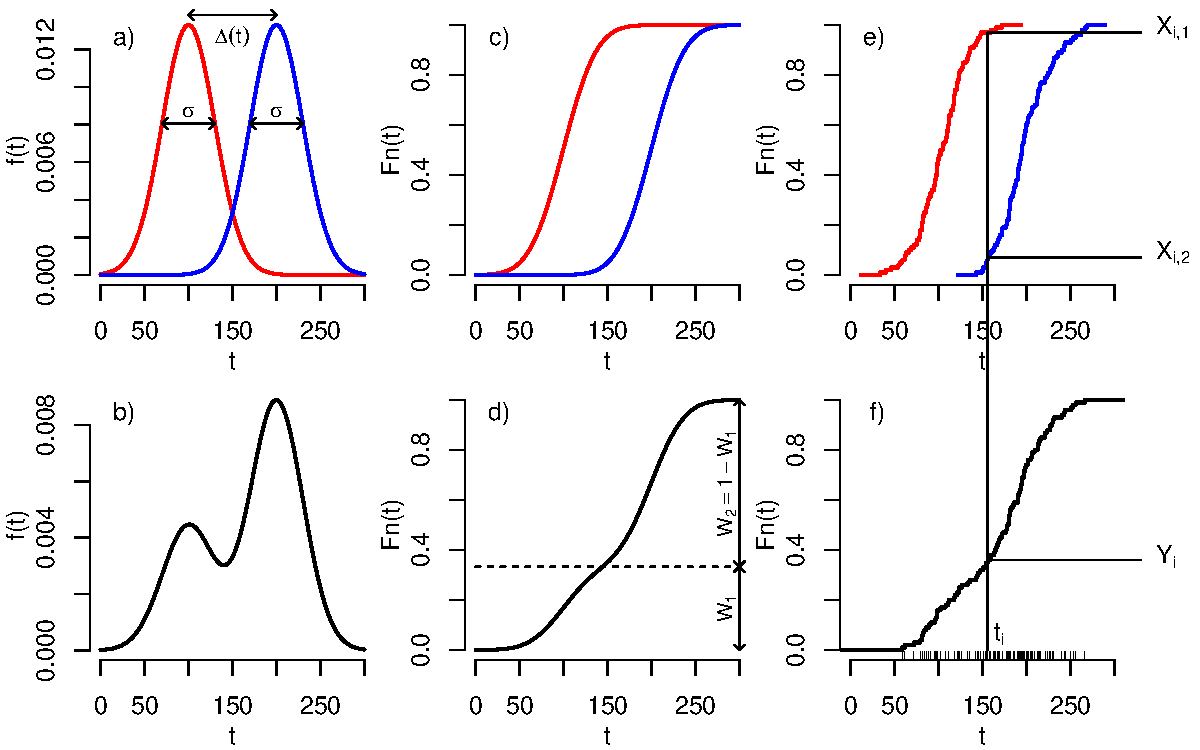
\includegraphics[width=.75\linewidth]{algorithm.pdf}
\captionof{figure}{Schematic overview of the mixing problem using a
  bivariate mixture of normal distributions as an example. a) density
  functions of two synthetic source populations, and b) a 1/2-mixture
  of these sources (i.e., $W_1=1/3$ and $W_2=2/3$). c) and d) are the
  corresponding cumulative distributions.  e) and f) are empirical
  cumulative distribution functions of random samples of 100 values
  from each of the three populations. $X_{1,i}$, $X_{2,i}$ and $Y_{i}$
  are the cumulative probabilities under the source and sink
  distributions for the $i$\textsuperscript{th} measurement.  These
  values are used to populate Equation~\ref{eq:unmix}.}
\label{fig:algorithm}

\section{Examples}\label{sec:examples}

As a first example, consider a binary mixture of two normal
distributions with the same standard deviation $\sigma$
(Figure~\ref{fig:algorithm}a). Let $\Delta(t)$ denote the lateral
separation between the two source distributions. When $\Delta(t)$ is
much larger than $\sigma$, the sink distribution is bimodal, making
the mixing proportions easy to recover. As $\Delta(t)$ decreases, the
sink becomes unimodal, making the deconvolution problem more
difficult. Figure~\ref{fig:bootstrap} shows the bootstrapped 95\%
confidence intervals for $W_1$ as $\Delta(t)$ varies from 0 to 3
standard deviations. As expected, the uncertainties decrease with
increasing separation. Nevertheless, the direct solution remains
accurate even when $\Delta(t)$ is small.\medskip

\noindent\begin{minipage}{.4\linewidth}
  \noindent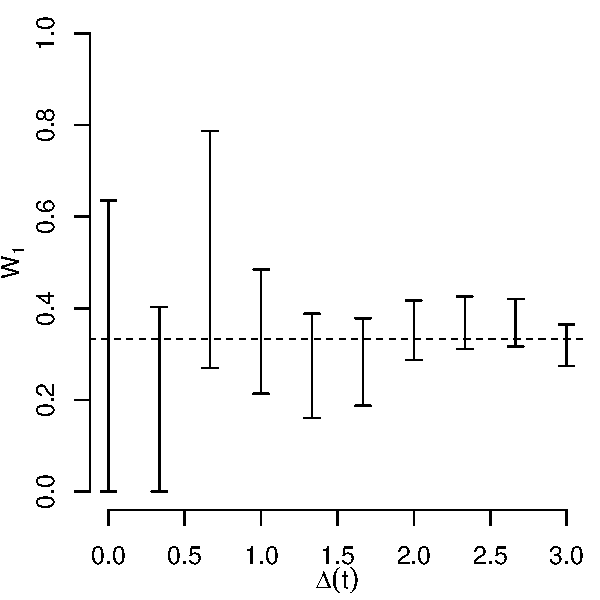
\includegraphics[width=\linewidth]{bootstrap.pdf}\medskip
\end{minipage}
\noindent\begin{minipage}{.6\linewidth}
\captionof{figure}{Bootstrapped 95\% confidence intervals for the
  mixing proportion of synthetic samples formed by 1/2 mixtures of two
  normal distributions with offset $\Delta(t)$, which is expressed as
  a number of standard deviations. The dashed line shows the true
  value for the mixing proportion $W_1$.}
\label{fig:bootstrap}
\end{minipage}

Figure~\ref{fig:Sickmann} applies the direct solution to the detrital
zircon U--Pb dataset of \citet{sickmann2016}, which was used as a case
study in the unmixing study of \citet{sharman2017}. The dataset
comprises seventeen sand samples from central California (USA): five
river samples, four beach samples and eight submarine canyon
samples. \citet{sharman2017} partitioned these data into three sources
(P1, P2 and P3) and twelve sinks. We retain the same partitioning to
facilitate comparison between the direct solution and the exhaustive
search algorithm of \citet{sharman2017}.\medskip

Figure~\ref{fig:Sickmann} consists of three parts. The top panel shows
the empirical cumulative distributions of the three sources. P1 and P2
have broad U--Pb age distributions, whereas P3 is more concentrated in
the 80--100\,Ma interval. The left-hand panels show the observed ($Y$,
red) and fitted ($X\hat{W}$, blue) distributions for each of the
twelve sinks. The goodness of fit is quantified using the
Cram\'{e}r--von Mises statistic (CvM), with higher values indicating a
poorer fit. Sample GSB has the highest CvM value in
Figure~\ref{fig:Sickmann}. Closer inspection reveals that its DZ dates
span a much narrower range than those of any of the three sources,
explaining the poor fit. Thus, the CvM statistic provides a useful
diagnostic for identifying potential problems with the unmixing
solution. Finally, the lower-right panel shows the estimated mixing
proportions for all twelve sinks.\medskip

Before comparing the direct solution with the exhaustive search
algorithm of \citet{sharman2017}, it is worth noting that the results
of the latter depend on the objective function used for
optimisation. \citet{sharman2017} explored five dissimilarity
functions (likeness, similarity, cross-correlation,
Kolmogorov--Smirnov and Kuiper), each yielding different results. They
illustrate this sensitivity using sample MAN, for which the estimated
mixing proportions span the following ranges across the five
functions: $66\%\leq{W_1}\leq{86\%}$, $3\%\leq{W_2}\leq{15\%}$ and
$0\%\leq{W_3}\leq{31\%}$. By comparison, the direct solution for MAN
yields $\{W_1=83\%,W_2=5\%,W_3=12\%\}$, with 95\% confidence intervals
of $66\%\leq{W_1}\leq{90\%}$, $0\%\leq{W_2}\leq{20\%}$ and
$0\%\leq{W_3}\leq{31\%}$. These confidence intervals encompass the
full range of solutions obtained by \citet{sharman2017}, while
avoiding the ambiguity introduced by the choice of dissimilarity
function.

\noindent\begin{minipage}{.5\linewidth}
  \noindent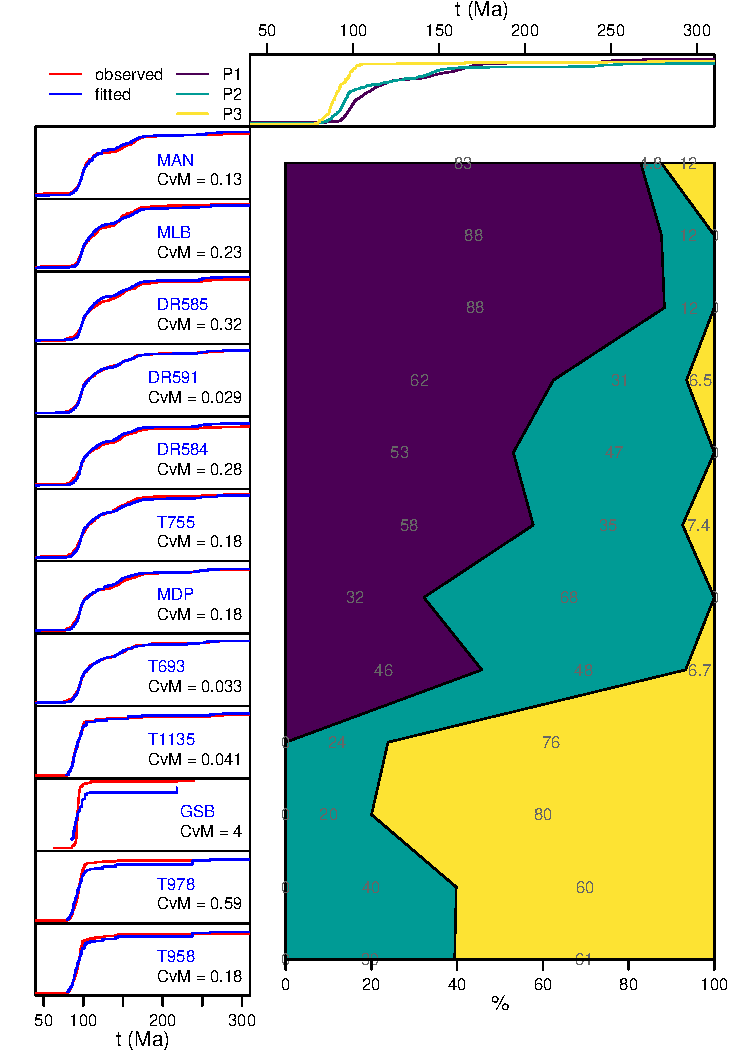
\includegraphics[width=\linewidth]{Sickmann.pdf}\medskip
\end{minipage}
\noindent\begin{minipage}{.5\linewidth}
\captionof{figure}{Unmixing the detrital zircon U--Pb dataset of
  \citet{sickmann2016}. The top and left margins show the three
  sources (P1, P2 and P3) are twelve sinks, respectively. `CvM' is
  the Cram\'{e}r--von Mises misfit of the optimal fit. The main panel
  shows the mixing proportions of the different samples.}
\label{fig:Sickmann}
\end{minipage}

\section{Implementation in IsoplotR}\label{sec:IsoplotR}

The new algorithm was implemented in the \texttt{R} package
\texttt{IsoplotR} (version 7.1 and higher) via a new \texttt{unmix}
function. It uses a modified least squares algorithm that enforces a
unit sum of the mixing proportions with a Lagrange multiplier. If the
solution returns any value outside the unit interval, a fallback
solution uses the non-negative least squares algorithm of
\citet{lawson1995} with a penalty applied to the final row to enforce
the unit sum of the weights. The \texttt{unmix} function can either be
called from the \texttt{R} console, or from \texttt{IsoplotR}'s
graphical user interface (GUI), which is available online and offline
\citet{vermeesch2018c}. In the GUI, the unmixing functions can be
accessed by selecting `detritals' and `unmix' as top-level options. At
the console:

\begin{verbatim}
library(IsoplotR)
DZ <- read.data("Sickmann.csv",method="detritals")
unmix(DZ,source_names=c("P1","P2","P3"))
\end{verbatim}

To obtain bootstrapped confidence intervals:

\begin{verbatim}
fit <- unmix(DZ,source_names=c("P1","P2","P3"),boot=TRUE,plot=FALSE)
\end{verbatim}

\noindent which returns a list containing matrices called \texttt{W},
\texttt{ll} and \texttt{ul}, storing the mixing proportions and the
lower and upper limits of their confidence intervals, respectively.

\section{Conclusions}\label{sec:conclusions}

This paper introduced a direct solution to the top-down sediment
unmixing problem, which had previously been addressed using exhaustive
and random search algorithms. Whereas these numerical approaches
become progressively slower as the number of sources increases, the
direct solution can be computed almost instantaneously on any modern
computer. The algorithm can accommodate any number of sources,
provided that this number does not exceed the number of dates in the
sink.\medskip

Beyond its obvious speed advantage, the direct solution eliminates the
ambiguity associated with choosing between different objective
functions in iterative approaches, some of which lack a firm
statistical basis. Instead, the new algorithm uses least squares to
minimise a single, well-established objective function: the
Cram\'{e}r--von Mises (CvM) statistic. When applied to multiple sinks,
the CvM statistic can help identify problematic samples that cannot be
adequately reproduced by the specified sources. In principle, it can
also be used to formally test whether a sink represents a mixture of
those sources. However, such tests have limited practical value
because their outcomes depend strongly on sample size. Given a
sufficiently large sample, no geological sink will be an exact mixture
of a finite number of sources. The CvM statistic is therefore better
used as a relative measure of goodness of fit than as a basis for
calculating p-values \citep{vermeesch2018b}.\medskip

As with any top-down unmixing model, the reliability of the results
depends on the validity of the input. Whether the estimated mixing
proportions reflect geological reality or an analytical artefact
depends on the assumption that all relevant sources have been
identified. Moreover, even if this assumption holds, the estimated
weights quantify only the contributions of the datable mineral, not
the total sediment. Converting these proportions into sediment budgets
requires estimates of mineral fertility \citep{malusa2016}, which are
not always available in real-world studies.

\section*{Acknowledgments}

This work was initiated in response to a request from
\texttt{IsoplotR} user Estefany Villanueva-Garc\'{i}a. Andy Carter and
Guido Pastore are thanked for beta-testing the algorithm. This
research was supported by the Natural Environment Research Council
(grant no. NE/T001518/1).

\section*{Supplementary Information}

All the code and data to generate the figures in this paper are
available online at \url{https://github.com/pvermees/supplements}.

%\bibliographystyle{/home/pvermees/Dropbox/abbrvplainnat.bst}
%\bibliography{/home/pvermees/Dropbox/biblio.bib}

\begin{thebibliography}{8}
\providecommand{\natexlab}[1]{#1}
\providecommand{\url}[1]{\texttt{#1}}
\expandafter\ifx\csname urlstyle\endcsname\relax
  \providecommand{\doi}[1]{doi: #1}\else
  \providecommand{\doi}{doi: \begingroup \urlstyle{rm}\Url}\fi

\bibitem[Lawson and Hanson(1995)]{lawson1995}
Lawson, C.~L. and Hanson, R.~J.
\newblock \emph{Solving least squares problems}.
\newblock SIAM, 1995.

\bibitem[Malus{\`a} et~al.(2016)Malus{\`a}, Resentini, and
  Garzanti]{malusa2016}
Malus{\`a}, M., Resentini, A., and Garzanti, E.
\newblock Hydraulic sorting and mineral fertility bias in detrital
  geochronology.
\newblock \emph{Gondwana Research}, 31:\penalty0 1--19, 2016.

\bibitem[Saylor et~al.(2019)Saylor, Sundell, and Sharman]{saylor2019}
Saylor, J., Sundell, K., and Sharman, G.
\newblock {Characterizing sediment sources by non-negative matrix factorization
  of detrital geochronological data}.
\newblock \emph{Earth and Planetary Science Letters}, 512:\penalty0 46--58,
  2019.
\newblock ISSN 0012-821X.
\newblock \doi{https://doi.org/10.1016/j.epsl.2019.01.044}.
\newblock URL
  \url{https://www.sciencedirect.com/science/article/pii/S0012821X19300706}.

\bibitem[Sharman and Johnstone(2017)]{sharman2017}
Sharman, G.~R. and Johnstone, S.~A.
\newblock Sediment unmixing using detrital geochronology.
\newblock \emph{Earth and Planetary Science Letters}, 477:\penalty0 183--194,
  2017.

\bibitem[Sickmann et~al.(2016)Sickmann, Paull, and Graham]{sickmann2016}
Sickmann, Z.~T., Paull, C.~K., and Graham, S.~A.
\newblock {Detrital-zircon mixing and partitioning in fluvial to deep marine
  systems, central California, USA}.
\newblock \emph{Journal of Sedimentary Research}, 86\penalty0 (11):\penalty0
  1298--1307, 2016.

\bibitem[Sundell and Saylor(2017)]{sundell2017}
Sundell, K. and Saylor, J.~E.
\newblock {Unmixing detrital geochronology age distributions}.
\newblock \emph{Geochemistry, Geophysics, Geosystems}, 2017.

\bibitem[Vermeesch(2018{\natexlab{a}})]{vermeesch2018c}
Vermeesch, P.
\newblock {\texttt{IsoplotR}: a free and open toolbox for geochronology}.
\newblock \emph{Geoscience Frontiers}, 9:\penalty0 1479--1493,
  2018{\natexlab{a}}.
\newblock \doi{10.1016/j.gsf.2018.04.001}.

\bibitem[Vermeesch(2018{\natexlab{b}})]{vermeesch2018b}
Vermeesch, P.
\newblock {Dissimilarity measures in detrital geochronology}.
\newblock \emph{Earth-Science Reviews}, 178:\penalty0 310--321,
  2018{\natexlab{b}}.
\newblock \doi{10.1016/j.earscirev.2017.11.027}.

\end{thebibliography}


\end{document}
